\section{NP Problems}

\subsection{The decision Problems}
X is a set of strings, given a string s an algorithm A solves problem X: A(s) = yes iff $s \in X$.\\\\
\emph{Formal Definition}: Algorithm A runs in poly-time if for every string s, A(s) terminates in at most p(|s|) "steps", where p(⋅) is some polynomial.\\\\
\emph{P-Problems}:  Decision problems for which there is a poly-time algorithm.\\\\
\emph{Certifier}: Algorithm C(s, t) is a certifier for problem X if for every string s, $s \in X$ if there exists a string t such that C(s, t) = true.\\\\
\emph{Practial Defintion of Certifier}: Given an instance of problem P and a solution S, it's possible to check in polynomial time that S is a solution for P.\\\\
\emph{NP-Problems (Non-polynomial deterministic problems)}: Decision problems for which there exists a poly-time certifier.\\\\
\emph{EXP-Problems (Exponential Problems)}: Decision problems for which there exists an exponential-time algorithm.\\\\

\[P \subseteq NP \subseteq EXP\]

The proof for the problem above is very simple: every problem in P has a certificate that can return true in polinomial time, NP has a certificate that return true in exponential time.

\subsection{The Hamiltonian Cycle}
Given an undirected graph G = (V, E), does there exist a simple cycle C that visits every node?A certificate could be a permutation of the n nodes, then the certifier checks in poly-time the permutation contains each node in V exactly once, and that there is an edge between each pair of adjacent nodes in the permutation. We can conclude that HAM-CYCLE is in NP.

\begin{figure}[H]
    \centering
    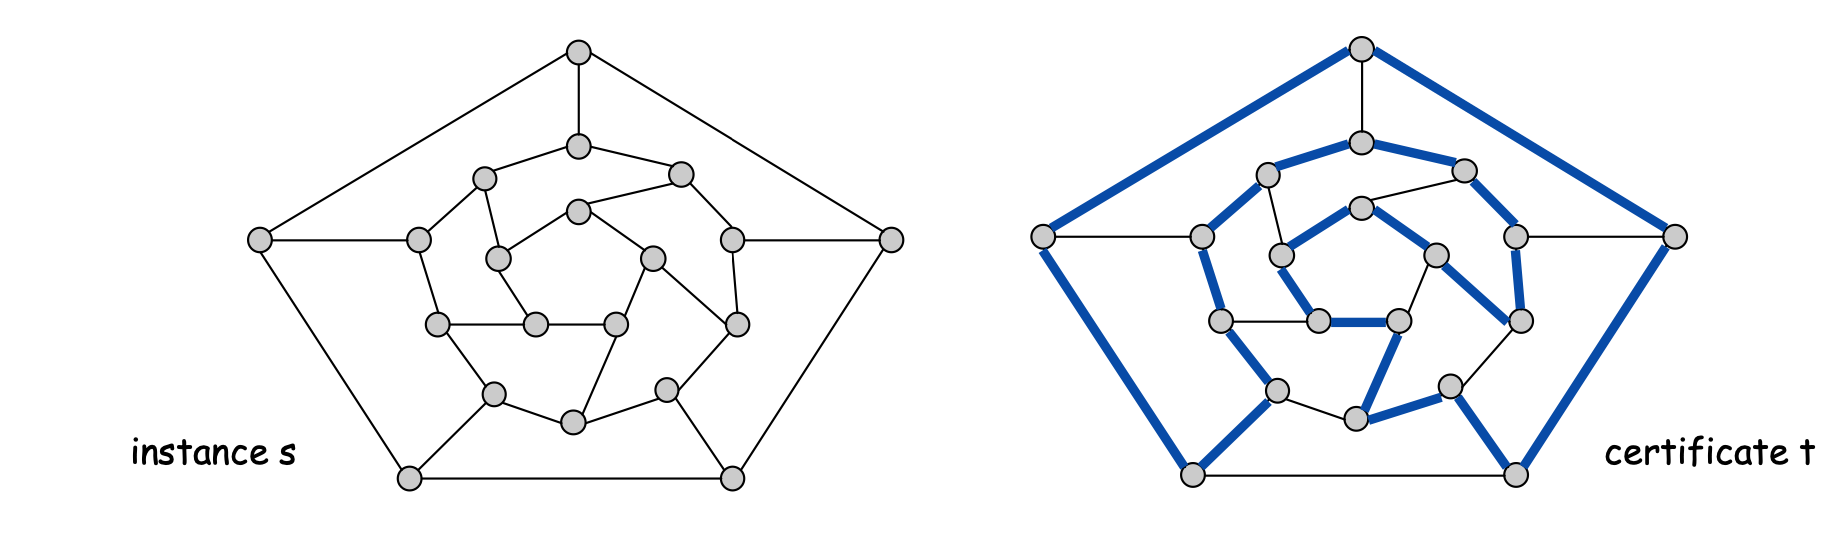
\includegraphics[width=0.6\textwidth ]{ham}
    \caption{Hamiltonian Cycle certification.}
\end{figure}

\clearpage

\subsection{NP Completeness}

A problem Y in NP with the property that for every problem X in NP, $X \leq _{p} Y$

\[NP \subseteq NP-Complete\]

\emph{Definition}:Problem X polynomial reduces (Cook) to problem Y if arbitrary instances of problem X can be solved using:Polynomial number of standard computational steps + Polynomial number of calls to oracle that solves problem Y.\\

\emph{Definition}:Problem X polynomial transforms (Karp) to problem Y if given any input x to X, we can construct an input y such that x is a yes instance of X if y is a true instance of Y.\\

Polynomial transformation is polynomial reduction with just one call to oracle for Y, exactly at the end of the algorithm for X. Almost all previous reductions were of this form.


\begin{figure}[H]
    \centering
    \includegraphics[width=0.7\textwidth ]{npComplete}
    \caption{Genealogy of most of the problems in NP}
\end{figure}

Fundamental NP-Complete Type of problems:
\begin{itemize}
    \item{Packing problems: SET-PACKING, INDEPENDENT SET}
    \item{Covering problems: SET-COVER, VERTEX-COVER}
    \item{Constraint satisfaction problems: SAT, 3-SAT}
    \item{Sequencing problems: HAMILTONIAN-CYCLE, TSP}
    \item{Partitioning problems: 3D-MATCHING 3-COLOR}
    \item{Numerical problems: SUBSET-SUM, KNAPSACK.}
\end{itemize}

\begin{figure}[H]
    \centering
    \includegraphics[width=0.4\textwidth ]{NPSet}
    \caption{Topology of NP problems}
\end{figure}

\clearpage